\chapter{Introduction to Neural Networks}

%\TODO{Chapter: Introduction}

\section{Biological Neurons}

Biological neurons are electrically excitable cells that are found in almost all
animals.
These neurons can transmit and receive electrical signals to one another via
synaptic connections, which maybe either excitatory or inhibitory.
Any given neuron will be either active or inactive depending on whether or not
its input exceeds a threshold.

\begin{center}
    \begin{tikzpicture}%[x=1pt,y=1pt]
    \newlength{\rs}
    \setlength{\rs}{1.5pt}
    % Nucleus
    \fill (0\rs,0\rs) circle (2\rs);
    % Soma
    \draw[thick] (0\rs,0\rs) circle (8\rs);
    % Dendrite
    \draw[thick] ( 45:8\rs) -- ( 45:16\rs);
        \draw[thick] ( 45:16\rs) -- ++(  0:4\rs);
        \draw[thick] ( 45:16\rs) -- ++( 90:4\rs);
    \draw[thick] ( 90:8\rs) -- ( 90:24\rs);
        \draw[thick] ( 90:16\rs) -- ++( 45:4\rs);
        \draw[thick] ( 90:16\rs) -- ++(135:4\rs);
        \draw[thick] ( 90:24\rs) -- ++( 45:8\rs);
        \draw[thick] ( 90:24\rs) -- ++(135:8\rs);
    \draw[thick] (135:8\rs) -- (135:24\rs);
        \draw[thick] (135:16\rs) -- ++( 90:4\rs);
        \draw[thick] (135:16\rs) -- ++(180:4\rs);
        \draw[thick] (135:24\rs) -- ++( 90:8\rs);
        \draw[thick] (135:24\rs) -- ++(180:8\rs);
    \draw[thick] (180:8\rs) -- (180:24\rs);
        \draw[thick] (180:16\rs) -- ++(135:4\rs);
        \draw[thick] (180:16\rs) -- ++(225:4\rs);
        \draw[thick] (180:24\rs) -- ++(135:8\rs);
        \draw[thick] (180:24\rs) -- ++(225:8\rs);
    \draw[thick] (225:8\rs) -- (225:24\rs);
        \draw[thick] (225:16\rs) -- ++(180:4\rs);
        \draw[thick] (225:16\rs) -- ++(270:4\rs);
        \draw[thick] (225:24\rs) -- ++(180:8\rs);
        \draw[thick] (225:24\rs) -- ++(270:8\rs);
    \draw[thick] (270:8\rs) -- (270:24\rs);
        \draw[thick] (270:16\rs) -- ++(225:4\rs);
        \draw[thick] (270:16\rs) -- ++(315:4\rs);
        \draw[thick] (270:24\rs) -- ++(225:8\rs);
        \draw[thick] (270:24\rs) -- ++(315:8\rs);
    \draw[thick] (315:8\rs) -- (315:16\rs);
        \draw[thick] (315:16\rs) -- ++(270:4\rs);
        \draw[thick] (315:16\rs) -- ++(360:4\rs);
    % Axon
    \draw[thick] (8\rs,0\rs) -- (12\rs,0\rs);
    \draw[thick,rounded corners=3\rs] (12\rs,-3\rs) rectangle (24\rs,3\rs);
        \fill (18\rs,0\rs) circle (1.5\rs);
    \draw[thick] (24\rs,0\rs) -- (26\rs,0\rs);
    \draw[thick,rounded corners=3\rs] (26\rs,-3\rs) rectangle (38\rs,3\rs);
        \fill (32\rs,0\rs) circle (1.5\rs);
    \draw[thick] (38\rs,0\rs) -- (40\rs,0\rs);
    \draw[thick,rounded corners=3\rs] (40\rs,-3\rs) rectangle (52\rs,3\rs);
        \fill (46\rs,0\rs) circle (1.5\rs);
    \draw[thick] (52\rs,0\rs) -- (54\rs,0\rs);
    \draw[thick,rounded corners=3\rs] (54\rs,-3\rs) rectangle (66\rs,3\rs);
        \fill (60\rs,0\rs) circle (1.5\rs);
    \draw[thick] (66\rs,0\rs) -- (68\rs,0\rs);
    \draw[thick,rounded corners=3\rs] (68\rs,-3\rs) rectangle (80\rs,3\rs);
        \fill (74\rs,0\rs) circle (1.5\rs);
    % Axon terminal
    \draw[thick] (80\rs,0\rs) -- (82\rs,0\rs);
        \draw[thick] (82\rs,0\rs) -- (86\rs,4\rs);
            \draw[thick] (86\rs,4\rs) -- (86\rs,7\rs);
            \draw[thick] (86\rs,4\rs) -- (89\rs,4\rs);
        \draw[thick] (82\rs,0\rs) -- (86\rs,-4\rs);
            \draw[thick] (86\rs,-4\rs) -- (86\rs,-7\rs);
            \draw[thick] (86\rs,-4\rs) -- (89\rs,-4\rs);
    % Labels
    % Soma
    \draw[latex'-] (65:9\rs) -- (65:36\rs);
    \node[anchor=south west,inner sep=1\rs] at (65:36\rs) {Soma};
    % Nucleus
    \draw[latex'-] (-65:3\rs) -- (-65:36\rs);
    \node[anchor=north west,inner sep=1\rs] at (-65:36\rs) {Nucleus};
    % Dendrite
    %\draw[latex'-] (225:25\rs) -- (225:36\rs);
    \draw[latex'-] (-17.7\rs,-25.7\rs) -- (-30\rs,-38\rs);
    \node[anchor=north east,inner sep=1\rs] at (-30\rs,-38\rs) {Dendrite};
    % Axon
    \draw[decorate,decoration={brace,raise=5\rs,amplitude=4\rs}] (12\rs,0\rs) -- (80\rs,0\rs);
    \node[anchor=south,inner sep=1\rs] at (46\rs,9\rs) {Axon};
    % Axon Terminal
    \draw[latex'-] (87\rs,8\rs) -- (95\rs,16\rs);
    \node[anchor=south west,inner sep=1\rs] at (95\rs,16\rs) {Axon Terminal};
\end{tikzpicture}

    \captionof{figure}{Diagram of a biological neuron.}
\end{center}

Signals are received by the neuron via connections to dendrites and soma.
If the threshold is met, electrical signals are sent along the axon to the
terminal, where it is connected to other neurons, or to a controllable cell such
as a neuromuscular junction.

%\TODO{Section: Biological Neurons}



\section{Artificial Intelligence}

The idea of artificial beings capable of human intelligence can be traced back
to mythical stories from ancient Greece.
One such story was that of a mythical automaton called Talos, who circled an
island's shores to protect it from pirates and other invaders.

In the $19^\text{th}$ century, other notions of artificial intelligence were
explored by fiction in stories such as Mary Shelley's ``Frankenstein'', and
Karel \v{C}apek's ``R.U.R.''.
Some of the fictional writings of the $20^\text{th}$ century further continued
exploring the concept in novels such as Isaac Asimov's ``I, Robot''.



Academic research into artificial intelligence began around the 1940's,
primarily due to findings in neurological research at the time.
The first explorations of artificial neural networks was done by
\cite{McCulloch:1943:Logical}, who investigated how simple logic functions
might be performed by idealised networks.
The neurons within these networks operated using some basic logic rules, applied
to a discrete time system which, can be summarised using the expression
\begin{align*}
    N(t) &= (E_1(t-1) \vee E_2(t-1) \vee \dots)
        \wedge \neg(I_1(t-1) \vee I_2(t-1) \vee \dots),
\end{align*}
where $N(t)$ is the state of a neuron at time $t$, and $E_i(t-1)$ and $I_i(t-1)$
are the states of the excitatory and inhibitory connections from the previous
time step respectively.
The result is such that the neuron will only be active if at least one
excitatory connection is active and all inhibitory connections are inactive.
The versatility of this definition is demonstrated in the following examples.
\begin{center}
    \begin{tabular}{ccc}
        SR Flip-flop & & AND Gate\\
        \begin{tikzpicture}
    [   neuron/.style=
        {   draw
        ,   regular polygon
        ,   regular polygon sides=3
        ,   shape border rotate=90
        ,   inner sep=2pt
        ,   node font=\small\ttfamily
        }
    ,   baseline=0pt
    ,   >={Stealth[scale=1.2]}
    ]
    \node[neuron] (S) at (0cm, 7mm) {S};
    \node[neuron] (R) at (0cm,-7mm) {R};
    \node[neuron] (M) at (2cm, 0cm) {M};
    \draw[->] (S) to[out=0,in=150] (M);
    \draw[-o] (R) to[out=0,in=180] (M);
    \draw[->] (M.east) .. controls (3cm,1cm) and (2cm,1cm) .. (M);
    \draw[->] (M.east) to (3cm,0cm);
\end{tikzpicture}
 & & \begin{tikzpicture}
    [   neuron/.style=
        {   draw
        ,   regular polygon
        ,   regular polygon sides=3
        ,   shape border rotate=90
        ,   inner sep=2pt
        ,   node font=\small\ttfamily
        }
    ,   baseline=0pt
    ,   >={Stealth[scale=1.2]}
    ]
    \node[neuron] (A) at (-2cm, 6mm) {A};
    \node[neuron] (B) at (-2cm,-6mm) {B};
    \node[neuron] (Af) at (0cm, 18mm) {1};
    \node[neuron] (Ab) at (0cm,  6mm) {2};
    \node[neuron] (Ba) at (0cm, -6mm) {3};
    \node[neuron] (Bf) at (0cm,-18mm) {4};
    \node[neuron] (R) at (2cm,0cm) {R};
    \draw[->] (A) to[out=0,in=240] (Af);
    \draw[->] (B) to[out=0,in=120] (Bf);
    \draw[->] (Af) to[out=0,in=120] (R);
    \draw[->] (Bf) to[out=0,in=240] (R);
    \draw[->] (A) to[out=0,in=120] (Ba);
    \draw[->] (B) to[out=0,in=240] (Ab);
    \draw[-o] (A) to[out=0,in=180] (Ab);
    \draw[-o] (B) to[out=0,in=180] (Ba);
    \draw[-o] (Ab) to[out=0,in=180] (R.west);
    \draw[-o] (Ba) to[out=0,in=180] (R.west);
\end{tikzpicture}
\\
        $\displaystyle N_M(t+1) = (N_S(t) \vee N_M(t)) \wedge\neg N_R(t)$ &
        &
        $\displaystyle N_R(t+2) = N_A(t) \vee N_B(t)$\\
    \end{tabular}
    \parbox{0.9\textwidth}{%
    \captionof{figure}{Two common logic circuits using McCulloch's neurons
    where the arrows and circles indicate excitatory and inhibitory
    connections respectively.}}
\end{center}
While this model provided insight into the mechanisms by which neurons operate,
the structure was static, and incapable of learning.



McCulloch's work was later cited by psychologist \cite{Hebb:1949:Organization},
as important for understanding how logical operations are performed; but
proposed that the structure of biological neurons was dynamic, not static, and
that frequently repeated stimuli caused gradual development.
At the scale of neuron, it was theorised that if one neuron successfully
excited another, the connection between them would strengthen, hence
increasing the likelihood that the former would be able to excite the latter
again in the future.
His theory was supported by research conducted by himself and others that showed
that intelligence-test performance in mature patients was often unaffected by
brain operations that would have prevented development in younger patients,
which suggested that learnt stimuli are processed differently to unknown
stimuli.
This hypothesis became known as Hebbian learning.



Computer simulations applying this theory to a small network were done by
\cite{Farley:1954:Simulation}.
The actions of the network were compared to that of a servo system which must
counteract any displacements so as to maintain a steady position.
The network was trained using a set of input patterns, which were subject to
non-linear transformations.
Similar to the Hebbian theory, when the network produces the correct responses,
the active connections are strengthened.
Although the results were of little neurophysiological significance, the results
were of great use for demonstrating computational simulations, which were
considerably slower at the time.

%\TODO{Section: Artificial Intelligence}



\subsection{Perceptrons}

The idea of the perceptron was originally conceived by
\cite{Rosenblatt:1958:Perceptron}, to represent a simplified model of
intelligent systems free from particularities of biological organisms, whilst
maintaining some of their fundamental properties.

The perceptron was built as a dedicated machine that consisted of a number of
photovoltaic cells, analogous to a retina, that feed into an``association
area''.
This association area contains a number of cells that each calculate a weighted
sum of the receptor values and output a signal if it exceeds a threshold.
Expressed mathematically, the output of a given association cell is given by
\begin{align*}
    A_i &= \begin{cases}
        1, & \sum_j w_{i,j}x_j > \theta\\
        0, & \text{otherwise}
    \end{cases},
\end{align*}
where $x_j$ is the value from the $j^\text{th}$ photovoltaic cell, $w_{i,j}$
is the weight of the connection between association cell $i$ and photovoltaic
cell $j$, and $\theta$ is the threshold.
These value weights were implemented using variable resistance wires that the
perceptron could adjust automatically.
The outputs from the association area are then connected to response cells,
which operate in a similar fashion to the association cells.
The activation of these response cells are the outputs of the perceptron, and
indicated the classification of the input.

Similar to \cite{Farley:1954:Simulation}, the method by which the perceptron
adjusted it weights was also based on which cells were active, and whether the
correct output was produced; except that the perceptron was also able to
``penalise'' weights when an incorrect result was outputted.

This machine was initially trained to reliably identify three different shapes:
a square, a circle, and a triangle; and did so with a better than chance
probability.
When attempting to use the perceptron for more complicated tasks, such as
character recognition, it failed to produce better than chance results.



After a decade of unsuccessful real world application attempts, a book titled
``\citetitle{Minsky:1969:Perceptrons}'' by \cite{Minsky:1969:Perceptrons}, was
released.
The book provided a rigorous mathematical analysis of the model, the results
showed that single layered, simple linear perceptron networks could not
calculate XOR predicates.
A 2017 reissue of the book contained a foreword by L\'eon Bottou, who wrote
``Their rigorous work and brilliant technique does not make the perceptron look
very good...''



Following the book's release, perceptron research effectively halted for 15
years until the first successful uses of multilayer networks by
\cite{McClelland:1986:Parallel}, which also served as a departure from the
neuron outputs being boolean values.
The multilayered structure of this new model allowed it to calculate the XOR
predicates that the single layer perceptrons could not.

The output of the units within these networks were defined by
\begin{align*}
    \Rvec{a}(t+1) &= \Rvec{F}(\Rvec{a}(t),\Rvec{net}_1(t),\Rvec{net}_2(t),...),
\end{align*}
where $\Rvec{net}_i$ is the $i^\text{th}$ propagation rule applied to the
inputs, $\Rvec{F}$ is the activation function, and $\Rvec{a}(t)$ is the
activation of the units at time step $t$.
The model usually uses a simplified version which can be summarised as
\begin{align*}
    a_i &= F\left(\sum_j w_{i,j}o_j\right),
\end{align*}
where $o_j$ is the output of unit $j$.
Hebbian learning could be performed the network by using iterative methods,
the most simple of which was given by
\begin{align*}
    \Delta w_{i,j} &= \eta\,a_i o_j,
\end{align*}
where $\eta$ is the learning rate, which is a constant.

%\TODO{Subsection: Perceptrons}



\subsection{Backpropagation}

In order for a neural network to learn, it must undergo some form of
optimisation process.
For the perceptron, this process was one of positive and negative reinforcement.



In the field of control theory, an optimisation method known as gradient descent
was developed by \cite{Kelley:1960:Gradient}, in which a given function of the
system is either maximised or minimised.
This is achieved by taking partial derivatives of the function with respect to
each parameter, which gives an approximation of how the function value will
change as the parameter changes.
By evaluating the partial derivatives, multiplying them by a constant, and
adding them to their respective parameters, the parameter values can be updated.
Using these new parameter values, one can expect to improve the function value.
This can be written as
\begin{align*}
    w_i' &= w_i + \eta\Rpdiff{f}{w_i}(\Rvec{x}),
\end{align*}
where $f(\Rvec{x})$ is the function to be optimised, $w_i$ is a parameter of
$f$, $w_i'$ is the updated parameter, and $\eta$ is ascent/descent parameter.
Positive $\eta$ values will maximise the function value, where as negative
values will minimise it.
The magnitude of $\eta$ determines the rate at which the method will attempt
change the parameters: if the value is too large, the method will overshoot the
optimal values; if the value is too small, the method will be too slow to
converge.

When this method was applied to neural networks, researchers sometimes
encountered an issue now known as the vanishing gradient problem.
A computer program will typically calculate the gradient via repeat applications
of chain rule; if there are many small terms, the gradient will tend to zero,
and the learning rate of the network will be minimal.



One of the methods that overcame this problem was developed by
\cite{Schmidhuber:1992:Compression}, where each layer of the network was
pre-trained to predict the next input from previous inputs.
Once each layer had been pre-trained, the network was then fine tuned using
backpropagation.
The method also provided a way of calculating which inputs were least expected,
so that more training time could be devoted to learning them.

Since then, computational power has significantly increased, and the slow
convergence caused by the vanishing gradient problem is less significant.
Further more, backpropagation and a simple variant the model outlined by
\cite{McClelland:1986:Parallel}, have become the standard for neural networks.
Namely
\begin{align*}
    x_i &= \phi\left(b_i + \sum_j w_{i,j} x_i\right),
\end{align*}
where $x_i$ is the output of neuron $i$, $w_{i,j}$ is the weight of connection
from $j$ to $j$, $b_i$ is the input bias of $i$, and $\phi$ is the activation
function.

%\TODO{Subsection: Backpropagation}



\section{Other Types of Artificial Neural Networks}

The preceding discussion has been focused on densely connected neural
networks, where each neuron in a layer is connected to every neuron in the
previous, but it is important to note, that many other neural network
architectures are often used together, and maybe more suitable under certain
contexts.

%\TODO{Section: Types of Neurons}



\subsection{Convolutional Neural Networks}

Many of the neural networks that had been employed for image recognition, such
as the preceptron, suffered from two major issues:
\begin{enumerate}
    \item processing high resolution images required each neuron in the first
        layer to be connected to every input, which caused the number of
        connections to become too large to process; and,
    \item most networks could not correctly identify an input if it was shifted.
\end{enumerate}
Similar to how biology inspired neural networks, findings in neurophysiology
inspired the architectures that would overcome these issues.
\cite{Hubel:1959:Receptive}, discovered that certain cells within a cat's
visual cortex would only respond to stimuli from specific regions of the retina.
Another important observation was that neighboring cells had overlapping
response regions.

Later research by \cite{Hubel:1962:Receptive}, also distinguished two categories
of cells termed:
``simple'', which had distinct excitatory and inhibitory connections, where
firing was maximised by slits at specific angles that passed through the centre;
and ``complex'', which could not be mapped out as trivial inhibitory/excitatory
regions, but were maximised slits at specific angles, regardless of position.



These findings inspired \cite{Fukushima:1980:Neocognitron}, to design the
neocognitron.
The neocognitron featured alternating layers of ``S-Planes'' and ``C-Planes'',
which were representations of the simple and complex cells respectively.
Each plane contains a number of feature maps, each unit within a feature map
is a function of a small region of the previous layer, a process now commonly
referred to as convolution.
S-Plane feature maps connect to all feature maps of the previous layer,
but C-Plane feature maps only connect to the corresponding feature map.
\begin{center}
    \HIDE{
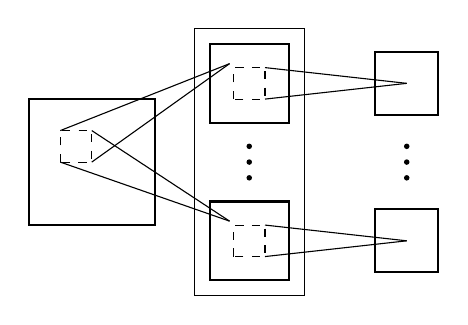
\begin{tikzpicture}
    \draw[thick] (-8mm,-8mm) rectangle (8mm,8mm);
    \draw[dashed] (-4mm, 0mm) rectangle (0mm,4mm);

    \draw[thick] (15mm,  5mm) rectangle ++(10mm,10mm);
    \foreach\y in {-2,0,2}
    {   \fill (20mm,1mm*\y) circle (1pt);
    }
    \draw[thick] (15mm,-15mm) rectangle ++(10mm,10mm);

    \draw (13mm,-17mm) rectangle (27mm,17mm);

    \draw (-4mm,4mm) -- (20mm-2.5mm, 10mm+2.5mm);
    \draw (20mm-2.5mm, 10mm+2.5mm) -- (0mm,0mm);
    \draw (0mm,4mm) -- (20mm-2.5mm,-10mm+2.5mm);
    \draw (20mm-2.5mm,-10mm+2.5mm) -- (-4mm,0mm);

    \draw[thick] (36mm, 6mm) rectangle ++(8mm,8mm);
    \foreach\y in {-2,0,2}
    {   \fill (40mm,1mm*\y) circle (1pt);
    }
    \draw[thick] (36mm,-14mm) rectangle (44mm,-6mm);

    \foreach\y in {-10,10}
    {   \draw[dashed] (18mm,1mm*\y-2mm) rectangle ++(4mm,4mm);
        \draw (22mm,1mm*\y+2mm) -- (40mm,1mm*\y);
        \draw (40mm,1mm*\y) -- (22mm,1mm*\y-2mm);
    }
\end{tikzpicture}
}
\begin{tikzpicture}
    [   kerline/.style =
        {   line join=round
        ,   densely dotted
        },
        kernel/.style =
        {   draw
        ,   circle
        ,   densely dotted
        }
    ]
    \newcommand{\kerlines}[2]{%
        \draw[kerline] (tangent cs:node=#1,point={(#2)},solution=1)
            -- (#2) -- (tangent cs:node=#1,point={(#2)},solution=2);
    }
    \newcommand{\kerdots}[1]{%
        \foreach\y in {-2,0,2}
        {   \fill (#1,1mm*\y) circle (1pt);
        }
    }

    %% planes
    % U0
    \node (U0) at ( 0mm,  0mm) [draw,rectangle,minimum size=20mm] {};
    % US1
    \node (US1G1) at (28mm,-15mm) [draw,rectangle,minimum size=16mm] {};
    \kerdots{28mm}
    \node (US1G2) at (28mm, 15mm) [draw,rectangle,minimum size=16mm] {};
    \draw (18mm,-25mm) rectangle (38mm,25mm);
    \node at (28mm,25mm) [above] {$U_{S1}$};
    % UC1
    \node (UC1G1) at (53mm,-15mm) [draw,rectangle,minimum size=14mm] {};
    \kerdots{53mm}
    \node (UC1G2)at (53mm, 15mm) [draw,rectangle,minimum size=14mm] {};
    \draw (44mm,-24mm) rectangle (62mm,24mm);
    \node at (53mm,24mm) [above] {$U_{C1}$};
    % US2
    \node (US2G1) at (75mm,-15mm) [draw,rectangle,minimum size=10mm] {};
    \kerdots{75mm}
    \node (US2G2) at (75mm, 15mm) [draw,rectangle,minimum size=10mm] {};
    \draw (68mm,-22mm) rectangle (82mm,22mm);
    \node at (75mm,22mm) [above] {$U_{S2}$};
    % UC2
    \node (UC2G1) at (94mm,-15mm) [draw,rectangle,minimum size=8mm] {};
    \kerdots{94mm}
    \node (UC2G2) at (94mm, 15mm) [draw,rectangle,minimum size=8mm] {};
    \draw (88mm,-21mm) rectangle (100mm,21mm);
    \node at (94mm,21mm) [above] {$U_{C2}$};

    %% kernels
    % U0 -> US1
    \coordinate (U0tUS1) at (-4mm,+4mm);
    \node[kernel] (U0K) at ($(U0)+(U0tUS1)$)
        [inner sep=0pt,minimum size=3mm] {};
    \coordinate (US1P1) at ($(US1G1)+(U0tUS1)$);
    \coordinate (US1P2) at ($(US1G2)+(U0tUS1)$);
    \kerlines{U0K}{US1P1}
    \kerlines{U0K}{US1P2}
    % US1 -> UC1
    \coordinate (US1tUC1) at (-4mm,-4mm);
    \node[kernel] (US1K1) at ($(US1G1)+(US1tUC1)$)
        [inner sep=0pt,minimum size=2mm] {};
    \node[kernel] (US1K2) at ($(US1G2)+(US1tUC1)$)
        [inner sep=0pt,minimum size=2mm] {};
    \coordinate (UC1P1) at ($(UC1G1)+(US1tUC1)$);
    \coordinate (UC1P2) at ($(UC1G2)+(US1tUC1)$);
    \kerlines{US1K1}{UC1P1}
    \kerlines{US1K2}{UC1P2}
    % UC1 -> US2
    \coordinate (UC1tUS2) at (-2mm,2mm);
    \node[kernel] (UC1K1) at ($(UC1G1)+(UC1tUS2)$)
        [inner sep=0pt,minimum size=3mm] {};
    \node[kernel] (UC1K2) at ($(UC1G2)+(UC1tUS2)$)
        [inner sep=0pt,minimum size=3mm] {};
    \coordinate (US2P1) at ($(US2G1)+(UC1tUS2)$);
    \coordinate (US2P2) at ($(US2G2)+(UC1tUS2)$);
    \kerlines{UC1K1}{US2P1}
    \kerlines{UC1K1}{US2P2}
    \kerlines{UC1K2}{US2P1}
    \kerlines{UC1K2}{US2P2}
    % US2 -> UC2
    \coordinate (US2tUC2) at (2mm,2mm);
    \node[kernel] (US2K1) at ($(US2G1)+(US2tUC2)$)
        [inner sep=0pt,minimum size=2mm] {};
    \node[kernel] (US2K2) at ($(US2G2)+(US2tUC2)$)
        [inner sep=0pt,minimum size=2mm] {};
    \coordinate (UC2P1) at ($(UC2G1)+(US2tUC2)$);
    \coordinate (UC2P2) at ($(UC2G2)+(US2tUC2)$);
    \kerlines{US2K1}{UC2P1}
    \kerlines{US2K2}{UC2P2}

    \foreach\x in {106,108,110}
    {   \fill (1mm*\x,0mm) circle (1pt);
    }
\end{tikzpicture}

    \captionof{figure}{Representation of the neocognitron's connectivity.}
\end{center}
Each layer of the network reduces the size of input image until the final layer
consists of single unit feature maps.
The network was originally trained to distinguish 5 digits, numbers 0 to 4,
using an unsupervised learning method, and was the first to reliably handle
shifted inputs.



\cite{Waibel:1989:Phoneme}, used concepts from the neocognitron to design the
time delay neural network, which was originally proposed for phoneme
recognition.
The networks were initially trained using backpropagation to detect and
distinguish between three acoustically similar phonemes (/b/, /d/, and /g/).
The model consisted of units similar to the neocognitron's S-Planes, where the
output of a unit is a function of a region from the previous layer.
The input for the model was a 2D spectrogram of an audio sample, with each
column representing a set of 16 spectral coefficients for a given time frame.

The first hidden layer contained columns of 8 units, each of which convolved the
spectral coefficients across 3 time frames, requiring a total of 384 weights.
Similarly, the second hidden layer contained columns of 3 units, each convolving
the previous layer across 5 time frames, requiring a total of 120 weights.
Finally, the output layer contains three units, each of which is a function of
the previous layer's corresponding row sum.
The most active unit is the phoneme present in the audio.

Once trained, the network was able to detect the correct phoneme, in real time,
under a variety of contexts, with an error of 1.5\%, a significant improvement
over the 6.3\% error from the most popular method at the time.



Similar techniques were used by \cite{LeCun:1989:Backpropagation}, to classify
handwritten digits.
A large number of 16 by 16 pixel images were used to train the network using
backpropagation.
The network consisted of two convolutional layers, and two dense layers.
Although the all of the units in a feature map shared the same weights, each
had a unique, adjustable bias.
Once trained, the network correctly classified 99.86\% of the training data, and
95\% of the test data.



This technique of combining convolutional and dense dense layers was also used
by \cite{Yamaguchi:1990:Neural}, for speech recognition.
Similar to \citeauthor{Waibel:1989:Phoneme}, the network takes a 2D spectrogram
as it's input and predicts which word was spoken.

The first layer, referred to as the event-net, convolves the input spectrogram
using a two layer subnetwork, which consists of a hidden partially connected
layer, and a fully connected single unit output layer.
Backpropagation is used to train each subnetwork of the event-net to only fire
when a word of the corresponding category is inputted.

The second layer, referred to as the time-alignment procedure, performs an
operation now known as max pooling, where each unit of the layer is the largest
value from the response region. If all the values are similar, use the one from
the middle of the search range; if all of the values are very low, the response
region size is increased

The third layer, referred to as the word-net, is another convolutional layer
using subnetwork, consisting of a fully connected layer, and a full connected
single unit output layer.
Backpropagation is used again in the same manner as in the event-net.

The forth layer, referred to as the super-net, is another convolutional
subnetwork that takes $N$ inputs and densely connects to $N+1$ outputs.
Each output corresponds to a word, except the last which denotes a rejected
result.

Finally, a decision algorithm compares the two highest outputs and rejects the
result if the difference does not exceed a preset threshold.



\subsection{Recurrent Neural Networks}

So far, the progression of time has been implemented as being another spacial
dimension.
Although this methodology proved effective for phoneme recognition tasks, it did
not work for other, more advanced temporal tasks.



\cite{Jordan:1986:Serial}, noted that representing time as a spacial dimension
required the network inputs to be stored in a buffer.
This buffer storage method was susceptible to a number of problems, including:
\begin{itemize}
    \item inability to account for input errors,
    \item lack of distinction between relative positions,
    \item difficulty with repeated actions, and
    \item difficulty processing different orderings of the same actions.
\end{itemize}
He proposed an alternative architecture, where the network takes the temporal
input in serial, whilst modifying its internal state.
This internal state is implemented by introducing cycles and delays into the
network.
Any network containing one or more cycles is described as being recurrent.

Such a network was initially trained to measure 8 phonetic features across time.
The input layer contained two groups of units:
input units, providing data from the current time frame;
and state units, providing compressed data from all previous time frames.
A hidden layer connects fully to all units from both groups in the input layer.
The output layer connects fully to the hidden layer.
The state units are connected to the output units and to themselves.
\begin{center}
    \begin{tikzpicture}
    [   > = {Stealth[scale=1.2]}
    ,   neuron/.style =
        {   draw
        ,   circle
        ,   inner sep = 0mm
        ,   outer sep = 0mm
        ,   minimum size = 7mm
        }
    ]
    \foreach\x in {0,1}
    {   \node[neuron] (I\x) at (\x*20mm-30mm, 0mm) {I\x};
        \node[neuron] (S\x) at (\x*20mm+10mm, 0mm) {S\x};
        \node[neuron] (H\x) at (\x*20mm-10mm,20mm) {H\x};
        \node[neuron] (O\x) at (\x*20mm-10mm,40mm) {O\x};
    }
    \foreach\x in {0,1}
    {   \foreach\y in {0,1}
        {   \draw[->] (I\x) to (H\y);
            \draw[->] (S\x) to (H\y);
            \draw[->] (H\x) to (O\y);
        }
        \draw[<-] (I\x) to ++(0mm,-20mm);
        \draw[->] (O\x) to ++(0mm, 20mm);
        \draw[->] (O\x) to[out=0,in=45] (S\x);
        \draw[->] (S\x) .. controls +( 5mm,-10mm) and +(-5mm,-10mm) .. (S\x);
    }

\end{tikzpicture}

    \captionof{figure}{Example of Jordan's recurrent neural network.}
\end{center}
During training, the network was exposed to one utterance at a time, and trained
to output the corresponding measures for each time frame.
For some combinations phonemes and features, any value is acceptable, these were
marked as ``don't-care'', and did not affect the error.
Due to the recurrent nature of the network, weight values were only updated
every 4 time steps.
The network learnt to process utterances and produce feature graphs that could
be used to identify the correct phonemes.



% \cite{Robinson:1987:Utility}
% based on control theory
% letter to word conversion
%   26 input, one for each letter
%   34 hidden
%   34 state
%    8 output, one for each word
%   learnt to output word at the start of the first letter of next word
% might not include



\cite{Elman:1990:Finding}, expanded Jordan's critiques of buffer-based
techniques by noting that there was no evidence of any biological equivalent.
He proposed that the state units should correspond to the hidden layer instead.
For each unit in the hidden layer, there is a corresponding state unit, which
holds the previous value of the hidden unit.
Units in the hidden layer is connected to the corresponding state unit, and
fully to the previous layer.
\begin{center}
    \begin{tikzpicture}
    [   > = {Stealth[scale=1.2]}
    ,   neuron/.style =
        {   draw
        ,   circle
        ,   inner sep = 0mm
        ,   outer sep = 0mm
        ,   minimum size = 7mm
        }
    ]
    \foreach\x in {0,1}
    {   \node[neuron] (I\x) at (20mm*\x, 0mm) {I\x};
        \node[neuron] (H\x) at (20mm*\x,20mm) {H\x};
        \node[neuron] (S\x) at (20mm*\x+40mm,20mm) {S\x};
        \node[neuron] (O\x) at (20mm*\x,40mm) {O\x};
    }
    \foreach\x in {0,1}
    {   \foreach\y in {0,1}
        {   \draw[->] (I\x) to (H\y);
            \draw[->] (H\x) to (O\y);
        }
        \draw[->] (H\x) to[out= 45,in=135] (S\x);
        \draw[->] (S\x) to[out=225,in=315] (H\x);
        \draw[<-] (I\x) to ++(0mm,-20mm);
        \draw[->] (O\x) to ++(0mm, 20mm);
    }

\end{tikzpicture}

    \captionof{figure}{Example of Elman's recurrent neural network.}
\end{center}
The network structure was initially used to predict sequential bit patterns.
In one such experiment, a number of random sentences were generated using a
small lexicon, and were presented to a network one character at a time without
breaks.
Each character was presented to the network as a 5-bit number, via 5 input
units.
The network processes this input using 20 hidden units each with a respective
state unit, and outputs a prediction of the next letter via 5 output units.

Once trained, the network struggled to predict the first letter of each randomly
selected word, but was able to accurately predict the letters that followed.



% \cite{Schmidhuber:1992:Learning}
% history compression
%   $o(t) = f(i(t),h(t))$, $h(t) = g(i(t-1),h(t-1))$
%   $o$ is output/prediction
%   $i$ is input
%   $h$ is hidden/internal state
%   $f$ and $g$ are functions
%\cite{Schmidhuber:1992:Learning} introduced the principle of history
%compression.
%A discrete time
%adaptive method for removing redundant information from sequences
%\begin{center}
%    \begin{tikzpicture}
    [   > = {Stealth[scale=1.2]}
    ,   func/.style=
        {   draw
        ,   circle
        ,   inner sep = 0mm
        ,   outer sep = 0mm
        ,   minimum size = 5mm
        }
    ,   bbox/.style=
        {   draw
        ,   rectangle
        ,   inner sep = 5mm
        }
    ]
    % box 0
    \node (B0) at (-30mm, 0mm) [bbox] {\phantom{\rule{30mm}{20mm}}};
    \node (F0) at (-30mm,-10mm) [func] {\small$f$};
    \node (G0) at (-15mm, 0mm) [func] {\small$g$};
    \node (I0) at (-30mm, 25mm) {$i(0)$};
    \node (O0) at (-30mm,-25mm) {$o(0)$};
    \draw[->] (B0.west) to[out=0,in=180] (F0);
    \draw[->] (B0.west) to (G0);
    \draw[->] (B0.north) to (F0);
    \draw[->] (B0.north) to[out=270,in=90] (G0);
    \draw[->] (I0) to (B0.north);
    \draw[->] (F0) to (O0);
    % box 1
    \node (B1) at (30mm, 0mm) [bbox] {\phantom{\rule{30mm}{20mm}}};
    \node (F1) at (30mm,-10mm) [func] {\small$f$};
    \node (G1) at (45mm, 0mm) [func] {\small$g$};
    \node (I1) at ( 30mm, 25mm) {$i(1)$};
    \node (O1) at ( 30mm,-25mm) {$o(1)$};
    \draw[->] (B1.west) to[out=0,in=180] (F1);
    \draw[->] (B1.west) to (G1);
    \draw[->] (B1.north) to (F1);
    \draw[->] (B1.north) to[out=270,in=90] (G1);
    \draw[->] (I1) to (B1.north);
    \draw[->] (F1) to (O1);
    % inter
    \node[above] (0mm,0mm) {h(1)};
    \node (H0) at (-70mm,0mm) {h(0)};
    \node (H2) at ( 70mm,0mm) {h(2)};
    \draw[->] (G0) to (B1.west);
    \draw[->] (H0) to (B0.west);
    \draw[->] (G1) to (H2);
\end{tikzpicture}

%    \captionof{figure}{Visualisation of history compression.}
%\end{center}



The recurrent neural networks previously described performed well for problems
with short time delays, but failed to perform tasks involving more than 10
discrete time steps.
The reason for this is the vanishing/exploding gradient problem.
Because errors backpropagate through the recurrent connections across multiple
time steps, the errors either tend towards zero or infinity.

A solution to this problem was proposed by \cite{Hochreiter:1997:Long}, where
the error term of the memory unit could be guaranteed to be a fixed constant.
This was achieved by using multiplicative gates to control the input and output
of the memory cell, resulting in a ``constant error carousel''.

Each cell took a weighted sum of the inputs and own previous state; and applied
a nonlinear function $g$ to obtain the net input signal, which connects to a
single, self-connected state unit.
A nonlinear function $h$ is applied to the value of the state unit to obtain
the output signal.
Gate units were controlled by taking a weighted sum of the layers inputs and
outputs, applying a nonlinear function, and multiplying by the relevant signal.
These gates prevented the network from perturbing its state, and prevents the
cell state from perturbing the reset of the network, allowing it to learn
long-lag-time tasks,
This new neural architecture was termed ``Long Short-Term Memory'' (LSTM).
% recurrent network architecture
% appropriate gradient-based learning algorithm
% variant of RTRL for learning



Although LSTM networks could learn long-lag-time tasks, they could not learn
certain, very long inputs that contain multiple sub-sequences.
This was because continual input streams would cause the cell state to grow
without bound, even in cases where the inputs suggest that the state should be
occasionally reset.
This problem was solved by \cite{Gers:1999:Learning}, by introducing a third
gate to the LSTM, which controlled the cell's internal recurrent connection.

It should be noted that an LSTM cell can learn to never forget, hence recovering
the previous model.
% LSTM fails to learn to correctly process certain very long or continual time
% series that are not a priori segmented into appropriate training subsequences
% with clearly defined beginnings and ends
% continual input stream eventually may cause the internal values of the cells
% to grow without bound, even if the repetitive nature of the problem suggests
% they should be reset occasionally
% introduced forget gate
% formulation allows for the network to learn to never forget inputs, hence new
% model is an expansion of the previous and can solve any problem that the
% previous could



A further expansion of the model by \cite{Gers:2000:Recurrent}, added
``peephole'' connections between the internal state unit and the gates, allowing
the gates to access the state, even when the output gate was closed.
Additionally, the output function, $h$, was removed, as there was no empirical
evidence to suggest it was required.

These peephole connections allowed the model to perform count and timing tasks,
such as producing nonlinear, precisely timed spikes.
\begin{center}
    \begin{tikzpicture}
    [   > = {Stealth}
    ,   neuron/.style =
        {   draw
        ,   circle
        ,   fill = white
        ,   inner sep = 2pt
        ,   outer sep = 0mm
        }
    ,   route/.style =
        {   draw
        ,   circle
        ,   fill = black
        ,   inner sep = 0mm
        ,   outer sep = 0mm
        ,   minimum size = 3pt
        }
    ,   phant/.style =
        {   inner sep = 0mm
        ,   outer sep = 0mm
        ,   minimum size = 0mm
        }
    ]
    \foreach\n in {0,1}
    {   \pgfmathtruncatemacro{\x}{70*\n-35}
        \draw (1mm*\x-20mm,-25mm) rectangle (1mm*\x+20mm,25mm);
        \node[phant] (L\n) at (1mm*\x-25mm,30mm) {};
        \node[phant] (R\n) at (1mm*\x+25mm,30mm) {};

        \node[neuron] (I\n) at (1mm*\x-10mm,-25mm) {\tiny$+$};
        \node[neuron] (F\n) at (1mm*\x-10mm,-17mm) {\tiny$g$};
        \draw[->] (I\n) to (F\n);
        \draw[<-] (I\n) to ++(0mm,-10mm);

        \node[route] (O\n) at (1mm*\x-10mm,25mm) {};
        \node[neuron] (G\n) at (1mm*\x-10mm,14mm) {\tiny$h$};
        \node[neuron] (OM\n) at (1mm*\x-10mm,20mm) {.};
        \draw[->] (G\n) to (OM\n);
        \draw[->] (OM\n) to (O\n);
        \draw[->] (O\n) to ++(0mm,10mm);

        \node[neuron] (IG\n) at (1mm*\x+20mm,-10mm) {\tiny$+$};
        \node[neuron] (IF\n) at (1mm*\x+13mm,-10mm) {\tiny$\sigma$};
        \node[neuron] (IM\n) at (1mm*\x-10mm,-10mm) {.};
        \draw[->] (IG\n) to (IF\n);
        \draw[->] (F\n) to (IM\n);
        \draw[->] (IF\n) to (IM\n);

        \node[neuron] (FG\n) at (1mm*\x+20mm,0mm) {\tiny$+$};
        \node[neuron] (FF\n) at (1mm*\x+13mm,0mm) {\tiny$\sigma$};
        \draw[->] (FG\n) to (FF\n);

        \node[neuron] (OG\n) at (1mm*\x+20mm,10mm) {\tiny$+$};
        \node[neuron] (OF\n) at (1mm*\x+13mm,10mm) {\tiny$\sigma$};
        \draw[->] (OG\n) to (OF\n);
        \draw[->] (OF\n) to[out=135,in=0] (OM\n);

        \node[neuron] (M\n) at (1mm*\x-10mm,0mm) {\tiny$+$};
        \node[neuron] (MM\n) at (1mm*\x+6mm,0mm) {.};
        \draw[->] (FF\n) to (MM\n);
        \draw[->] (M\n) to[out=45,in=135] (MM\n);
        \draw[->] (MM\n) to[out=225,in=315] (M\n);
        \draw[->] (IM\n) to (M\n);
        \draw[->] (M\n) to (G\n);

        \draw[-] (O\n) to[out=45,in=135] (R\n);
        \draw[->] (R\n) to[out=315,in=45] (IG\n);
        \draw[->] (R\n) to[out=315,in=45] (FG\n);
        \draw[->] (R\n) to[out=315,in=45] (OG\n);

        \draw[->] (O\n) .. controls +(-25mm,20mm) and +(-25mm,-20mm)  .. (I\n);
        \draw[->] (1mm*\x+30mm,-35mm) to[out=90,in=325] (IG\n);
        \draw[->] (1mm*\x+30mm,-35mm) to[out=90,in=325] (FG\n);
        \draw[->] (1mm*\x+30mm,-35mm) to[out=90,in=325] (OG\n);
        %peep hole connectionss
        \draw[->] (M\n) to[out=-67.5,in=135] (IG\n);
        \draw[->] (M\n) to[out=45,in=135] (FG\n);
        \draw[->] (M\n) to[out=45,in=135] (OG\n);
    }
    %\draw[-] (O1) to[out=135,in=45] (L1);
    %\draw[->] (L1) to[out=225,in=45] (IG0);
    %\draw[->] (L1) to[out=225,in=45] (FG0);
    %\draw[->] (L1) to[out=225,in=45] (OG0);
    \draw[-] (O0) to[out=45,in=135] (R1);
    \draw[->] (O1) to[out=135,in=45] (IG0);
    \draw[->] (O1) to[out=135,in=45] (FG0);
    \draw[->] (O1) to[out=135,in=45] (OG0);
    \node[anchor=west] (IL) at ($(IG1)+(15mm,0mm)$) {\tiny In gate};
    \node[anchor=west] (FL) at ($(FG1)+(15mm,0mm)$) {\tiny Forget gate};
    \node[anchor=west] (OL) at ($(OG1)+(15mm,0mm)$) {\tiny Out gate};
    \draw[densely dotted] (IL) to (IG1);
    \draw[densely dotted] (FL) to (FG1);
    \draw[densely dotted] (OL) to (OG1);
    \draw[densely dotted] (-55mm,-41mm) rectangle (75mm,-35mm);
    \node at (10mm,-38mm) {\tiny Previous layer};
\end{tikzpicture}

    \parbox{0.9\textwidth}{%
    \captionof{figure}{Visualisation of two LSTM units, where $\sigma$,
    $f$, and $g$ are function units;
    $+$ is a weighted summation unit; and $\cdot$ is multiply unit.}}
\end{center}
% during learning no error signals are propagated back from gates
% via peephole connections



